\section{Nullstellen}
Im Unterricht mag der Eindruck entstanden sein, dass man die meisten Gleichungen exakt lösen kann. Tatsächlich ist das aber eher die Ausnahme. So gibt es zum Beispiel keine Auflösungsformel für die Nullstellen von Polynomen vom Grad 5 oder höher. Auch viele andere Gleichungen lassen sich nicht unter Zuhilfenahme der elementaren Funktionen lösen – ein Beispiel dafür ist die Gleichung $e^x=10x$. In diesen Fällen ist man auf numerische Methoden angewiesen, mit welchen man die Lösung der Gleichung näherungsweise bestimmen kann.

Es gibt eine Vielzahl solcher numerischen Methoden. Alle haben gemeinsam, dass man bestimmte Rechenschritte wiederholt ausführt und somit in der Regel immer bessere Approximationen für die gesuchte Lösung findet. Weil sich ausserdem jede Gleichung in die Form $f(x) = 0$ bringen lässt, wird in den vorgestellten Methoden jeweils die Nullstelle einer Funktion gesuscht.

\subsection{Bisektionsverfahren}
Die Idee des Bisektionsverfahrens ist die Folgende: Wenn man bei einer stetigen Funktion $f$ zwei Stellen $x_1$ und $x_2$ findet, mit der Eigenschaft, dass $f(x_1)$ und $f(x_2)$ unterschiedliche Vorzeichen aufweisen, dann befindet sich mindestens eine Nullstelle von $f$ im Intervall $[x_1, x_2]$.

\begin{bsp}
	{Bisektionsverfahren}{Intro-Bisektion}
	Gegeben ist die Funktion $f(x) = x^3+5x-9$. Gesucht ist eine Nullstelle $x_0$.
	\begin{center}
		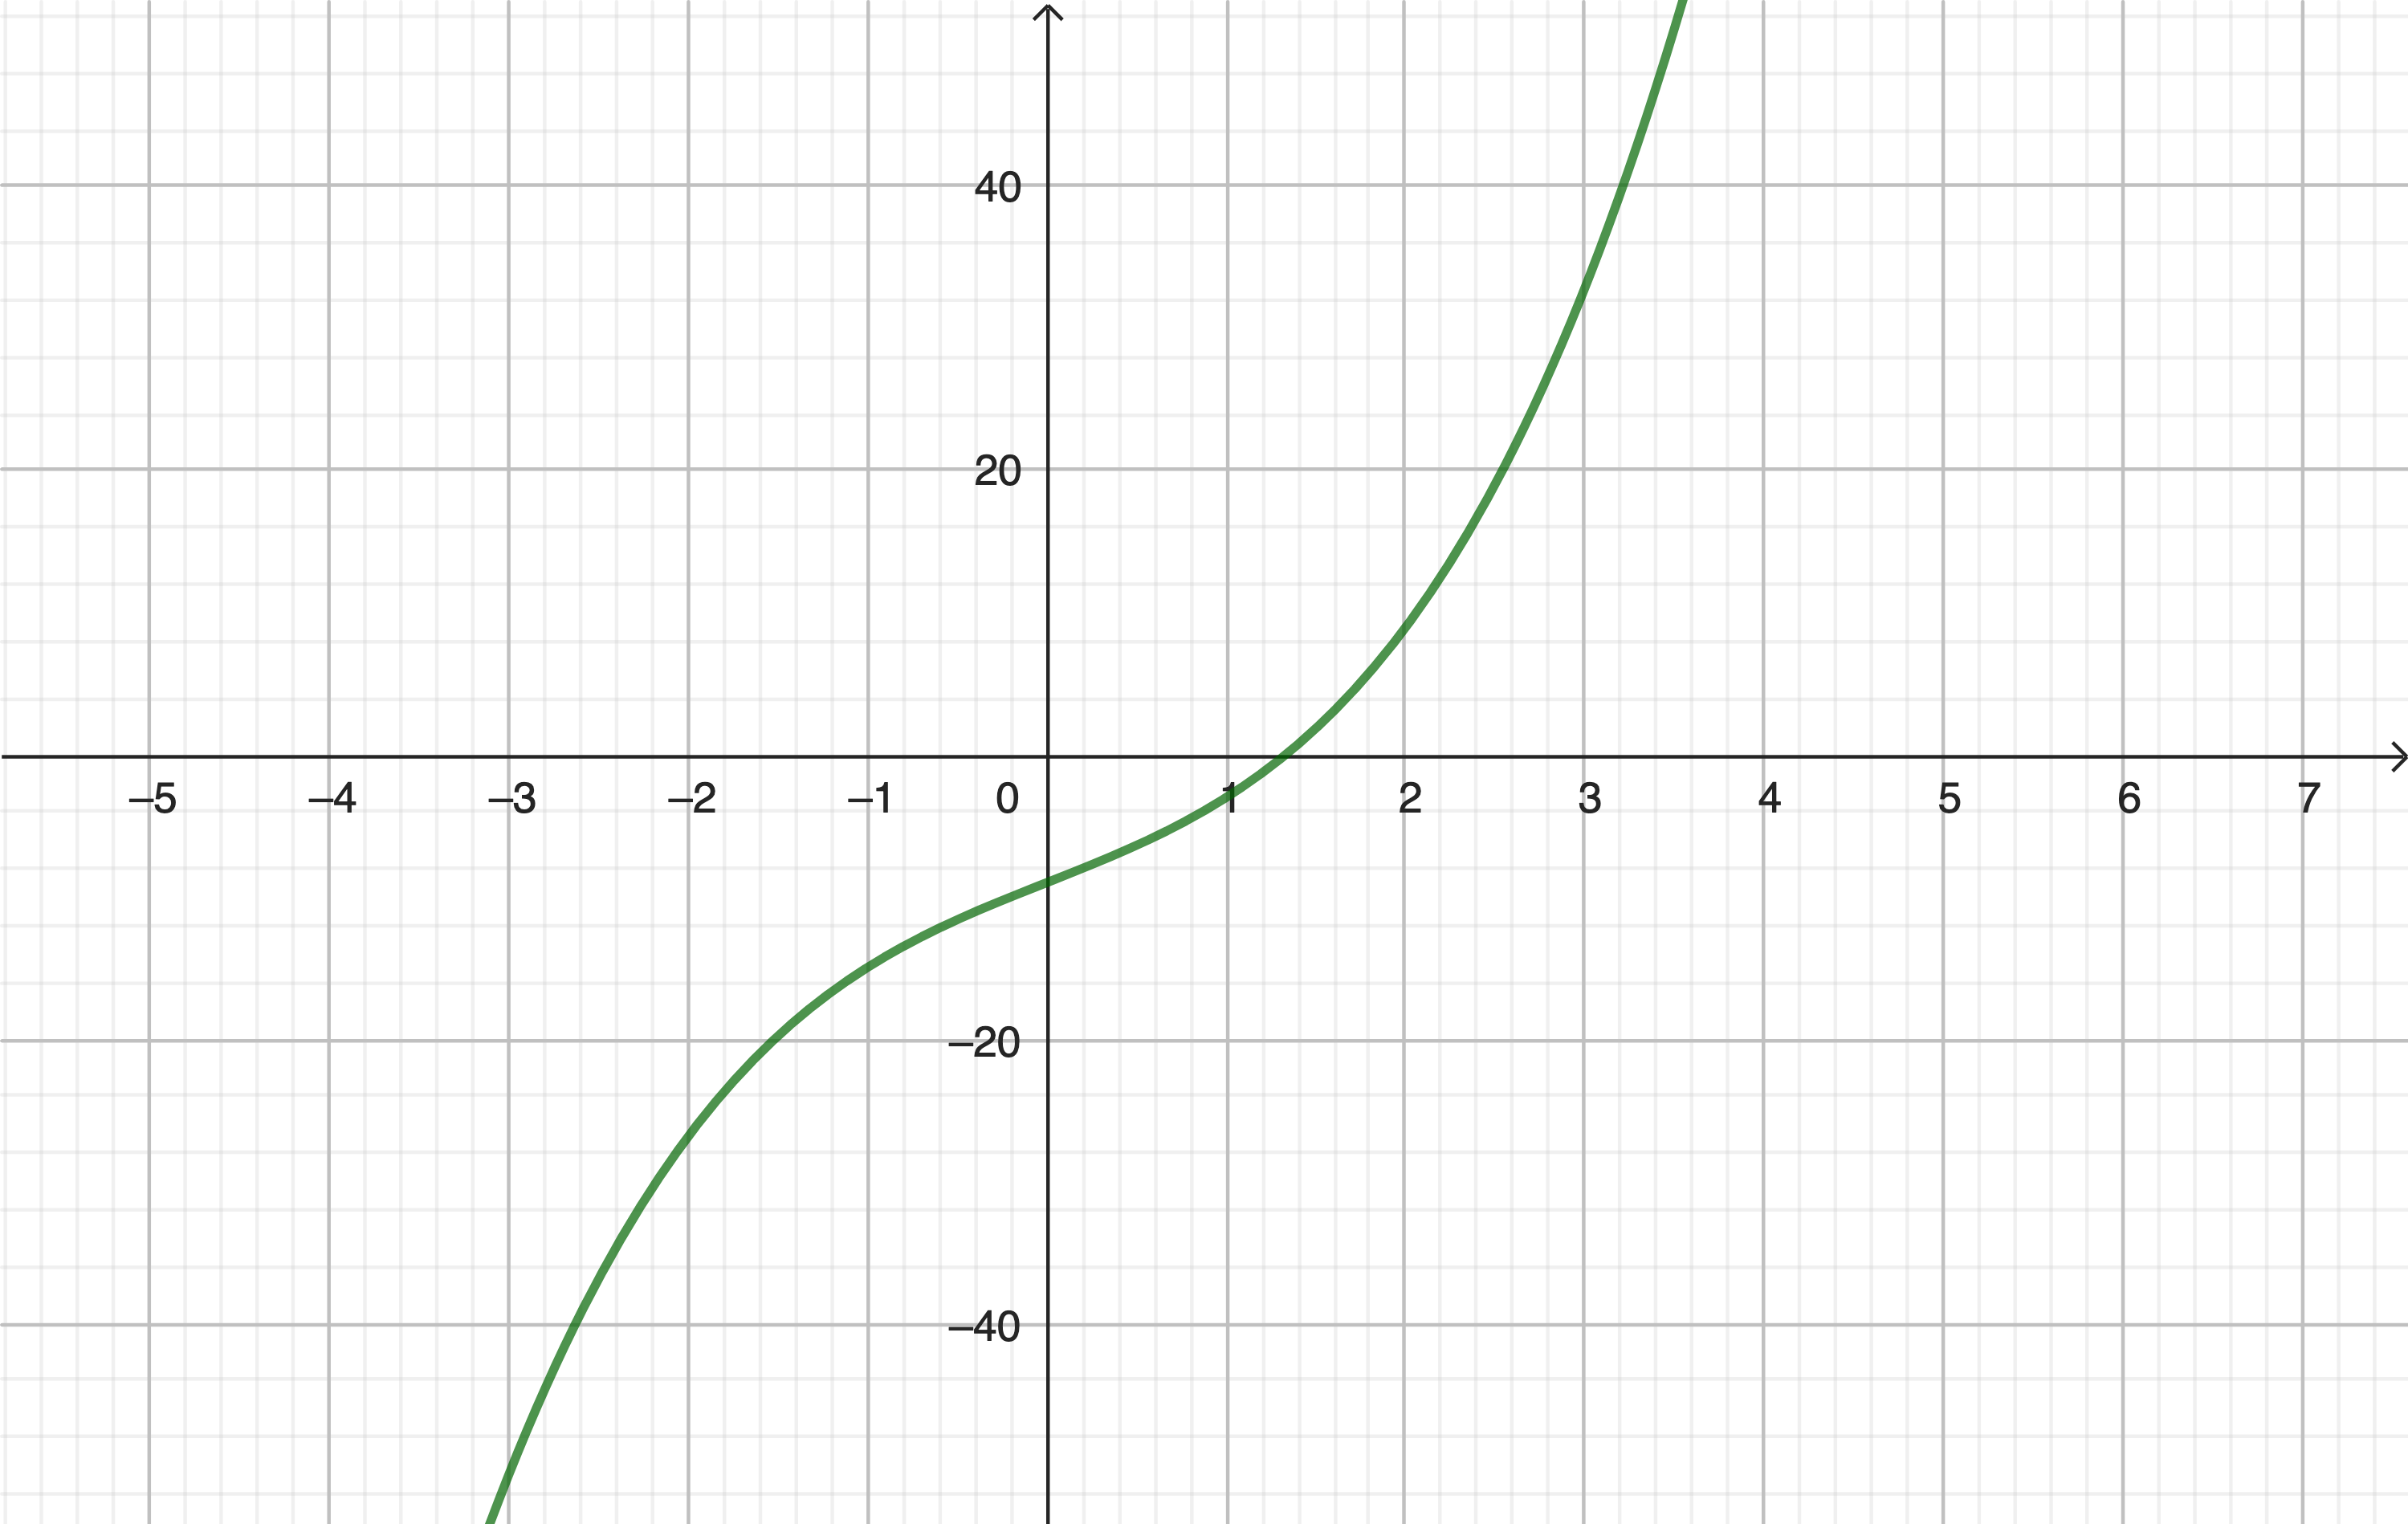
\includegraphics[width = 0.5\textwidth]{media/Bsp_Bisektion.png}
	\end{center}
	Wie man leicht nachrechnet ist
	\[ f(1) = 1+5-9 = -3, \qquad \text{und} \qquad f(2)=8+10-9=9 \]
	Also gibt es mindestens eine Nullstelle $x_0$ im Intervall $[1,2]$.

	Wir testen nun das Argument $x=1.5$ in der Mitte des Intervalls und erhalten
	\[ f(1.5) = 1.875.\]
	Wir stellen fest, dass $f(1.5)$ und $f(1)$ unterschiedliche Vorzeichen haben. Die Nullstelle liegt demnach im Bereich $1 < x_0 < 1.5$.

	Wir fahren nun wiederholt so fort, dass wir die die Mitte des Intervalls testen, in welchem die Nullstelle liegen kann. Nach jedem Schritt ersetzen wir das ursprüngliche Intervall durch diejenige Hälfte, deren Randpunkte unterschiedliche Vorzeichen besitzen.

	$f(1.25) \approx -0.8 \Rightarrow x_0 \in [1.25, 1.5]$.

	$f(1.375) \approx 0.5 \Rightarrow x_0 \in [1.25, 1.375]$.

	$f(1.3125) \approx -0.2 \Rightarrow x_0 \in [1.3125, 1.375]$.

	$f(1.34375) \approx 0.1 \Rightarrow x_0 \in [1.3125, 1.34375]$.

	Nach fünf Halbierungen wissen wir, dass die Nullstelle im Intervall $[1.3125,1.34375]$ liegt. Als Näherungswert können wir beispielsweise die Intervallmitte $x_0\approx 1.328125$ verwenden. Der Abstand zur richtigen Lösung ist dann höchstens so gross, wie die Hälfte der Intervallbreite $\frac{1.34375-1.3125}{2} = 0.015625$.
\end{bsp}

\begin{ueb}
	{Zum Bisektionsverfahren}{bisektion}
	\begin{enumerate}
		\item Führen Sie drei Schritte des Bisektionsverfahren durch, um eine Näherung für Lösung der Gleichung $e^x=10x$ im Intervall $[3,4]$ zu finden.
		\item Wie viele Schritte sind mindestens nötig, um eine Nullstelle einer Funktion $f(x)$ im Intervall $[0,4]$ auf eine Genauigkeit von $0.01$ zu finden.
		\item Ergänzen Sie das folgende Programm, um das Bisektionsverfahren in Python durchzuführen:
		      \lstinputlisting[language=Python]{Programme/bisektion.py}
		\item Testen Sie Ihr Programm auch mit der Gleichung aus Aufgabe 1. Dazu können Sie die Exponentialfunktion aus der Bibliothek \lstinline|math| wie folgt importieren: \lstinline|from math import exp|. Anschliessend kann man die Exponentialfunktion $e^x$ so verwenden: \lstinline|exp(x)|
		\item Ändern Sie das Programm so ab, dass nicht die Anzahl Schritte vorgegeben wird, sondern die Genauigkeit der Approximation.
	\end{enumerate}
\end{ueb}

\clearpage
\emph{Lösungen:}
\begin{enumerate}
	\item Nach drei Schritten beträgt die Approximation: $x_0 \approx 3.5625$
	\item Das Intervall wird in jedem Schritt halbiert. Nach $n$-Schritten beträgt die Breite $\frac{4-2}{2^n} = 2^{1-n}$. Die Genauigkeit ist dann die Hälfte der Intervallbreite, also $2^{-n}$. Also $2^{-n} = 0.01 \iff n = -\log_2(0.01) \approx 6.6$. Nach $n=7$ Schritten ist die gewünschte Genauigkeit erreicht.
	\item Mögliche Lösung:
	      \lstinputlisting[language=Python]{Programme/bisektion-lsg.py}
\end{enumerate}















\clearpage
\subsection{Lineare Interpolation – Regula Falsi}
Beim \Cref{bsp:Intro-Bisektion} zum Bisektionsverfahren haben wir aus $f(1)=-3$ und $f(2) = 9$ geschlossen, dass es eine Nullstelle zwischen diesen beiden Stellen gibt. Die Beträge der beiden Funktionswerte lassen jedoch weiter vermuten, dass die gesuchte Nullstelle näher bei $x=1$ als bei $x=2$ liegt, weil $|f(1)| < |f(2)|$.

Diese intuitive Idee wird durch die Regula Falsi\footnote{Der Name ist eine Kurzform von ``Regula duarum falsarum Positionum'', weil man aus zwei falschen Stellen eine bessere findet (Siehe: \href{https://de.wikipedia.org/wiki/Regula_falsi}{Wikipedia})} umgesetzt.
Die Grundidee besteht darin, die Funktion im betrachteten Intervall durch eine Gerade zu ersetzen und die Nullstelle dieser Geraden als Näherung für die tatsächliche Nullstelle zu verwenden.
Konkret wird im Beispiel eine Gerade zwischen den beiden Punkten $(1,-3)$ und $(2,9)$ gezogen und deren Schnittstelle mit der $x$-Achse berechnet:

\begin{bsp}
	{Regula Falsi}{intro-lineareInterpolation}
	Gegeben ist die Funktion $f(x) = x^3+5x-9$. Gesucht ist eine Nullstelle $x_0$.
	Wie man leicht nachrechnet ist
	\[ f(1) = 1+5-9 = -3, \qquad \text{und} \qquad f(2)=8+10-9=9 \]
	Also gibt es mindestens eine Nullstelle $x_0$ im Intervall $[1,2]$.

	Die Gerade zwischen den beiden Punkten $(1,-3)$ und $(2,9)$ hat die Steigung:
	\[ m = \frac{9-(-3)}{2-1} = 12\]
	\begin{center}
		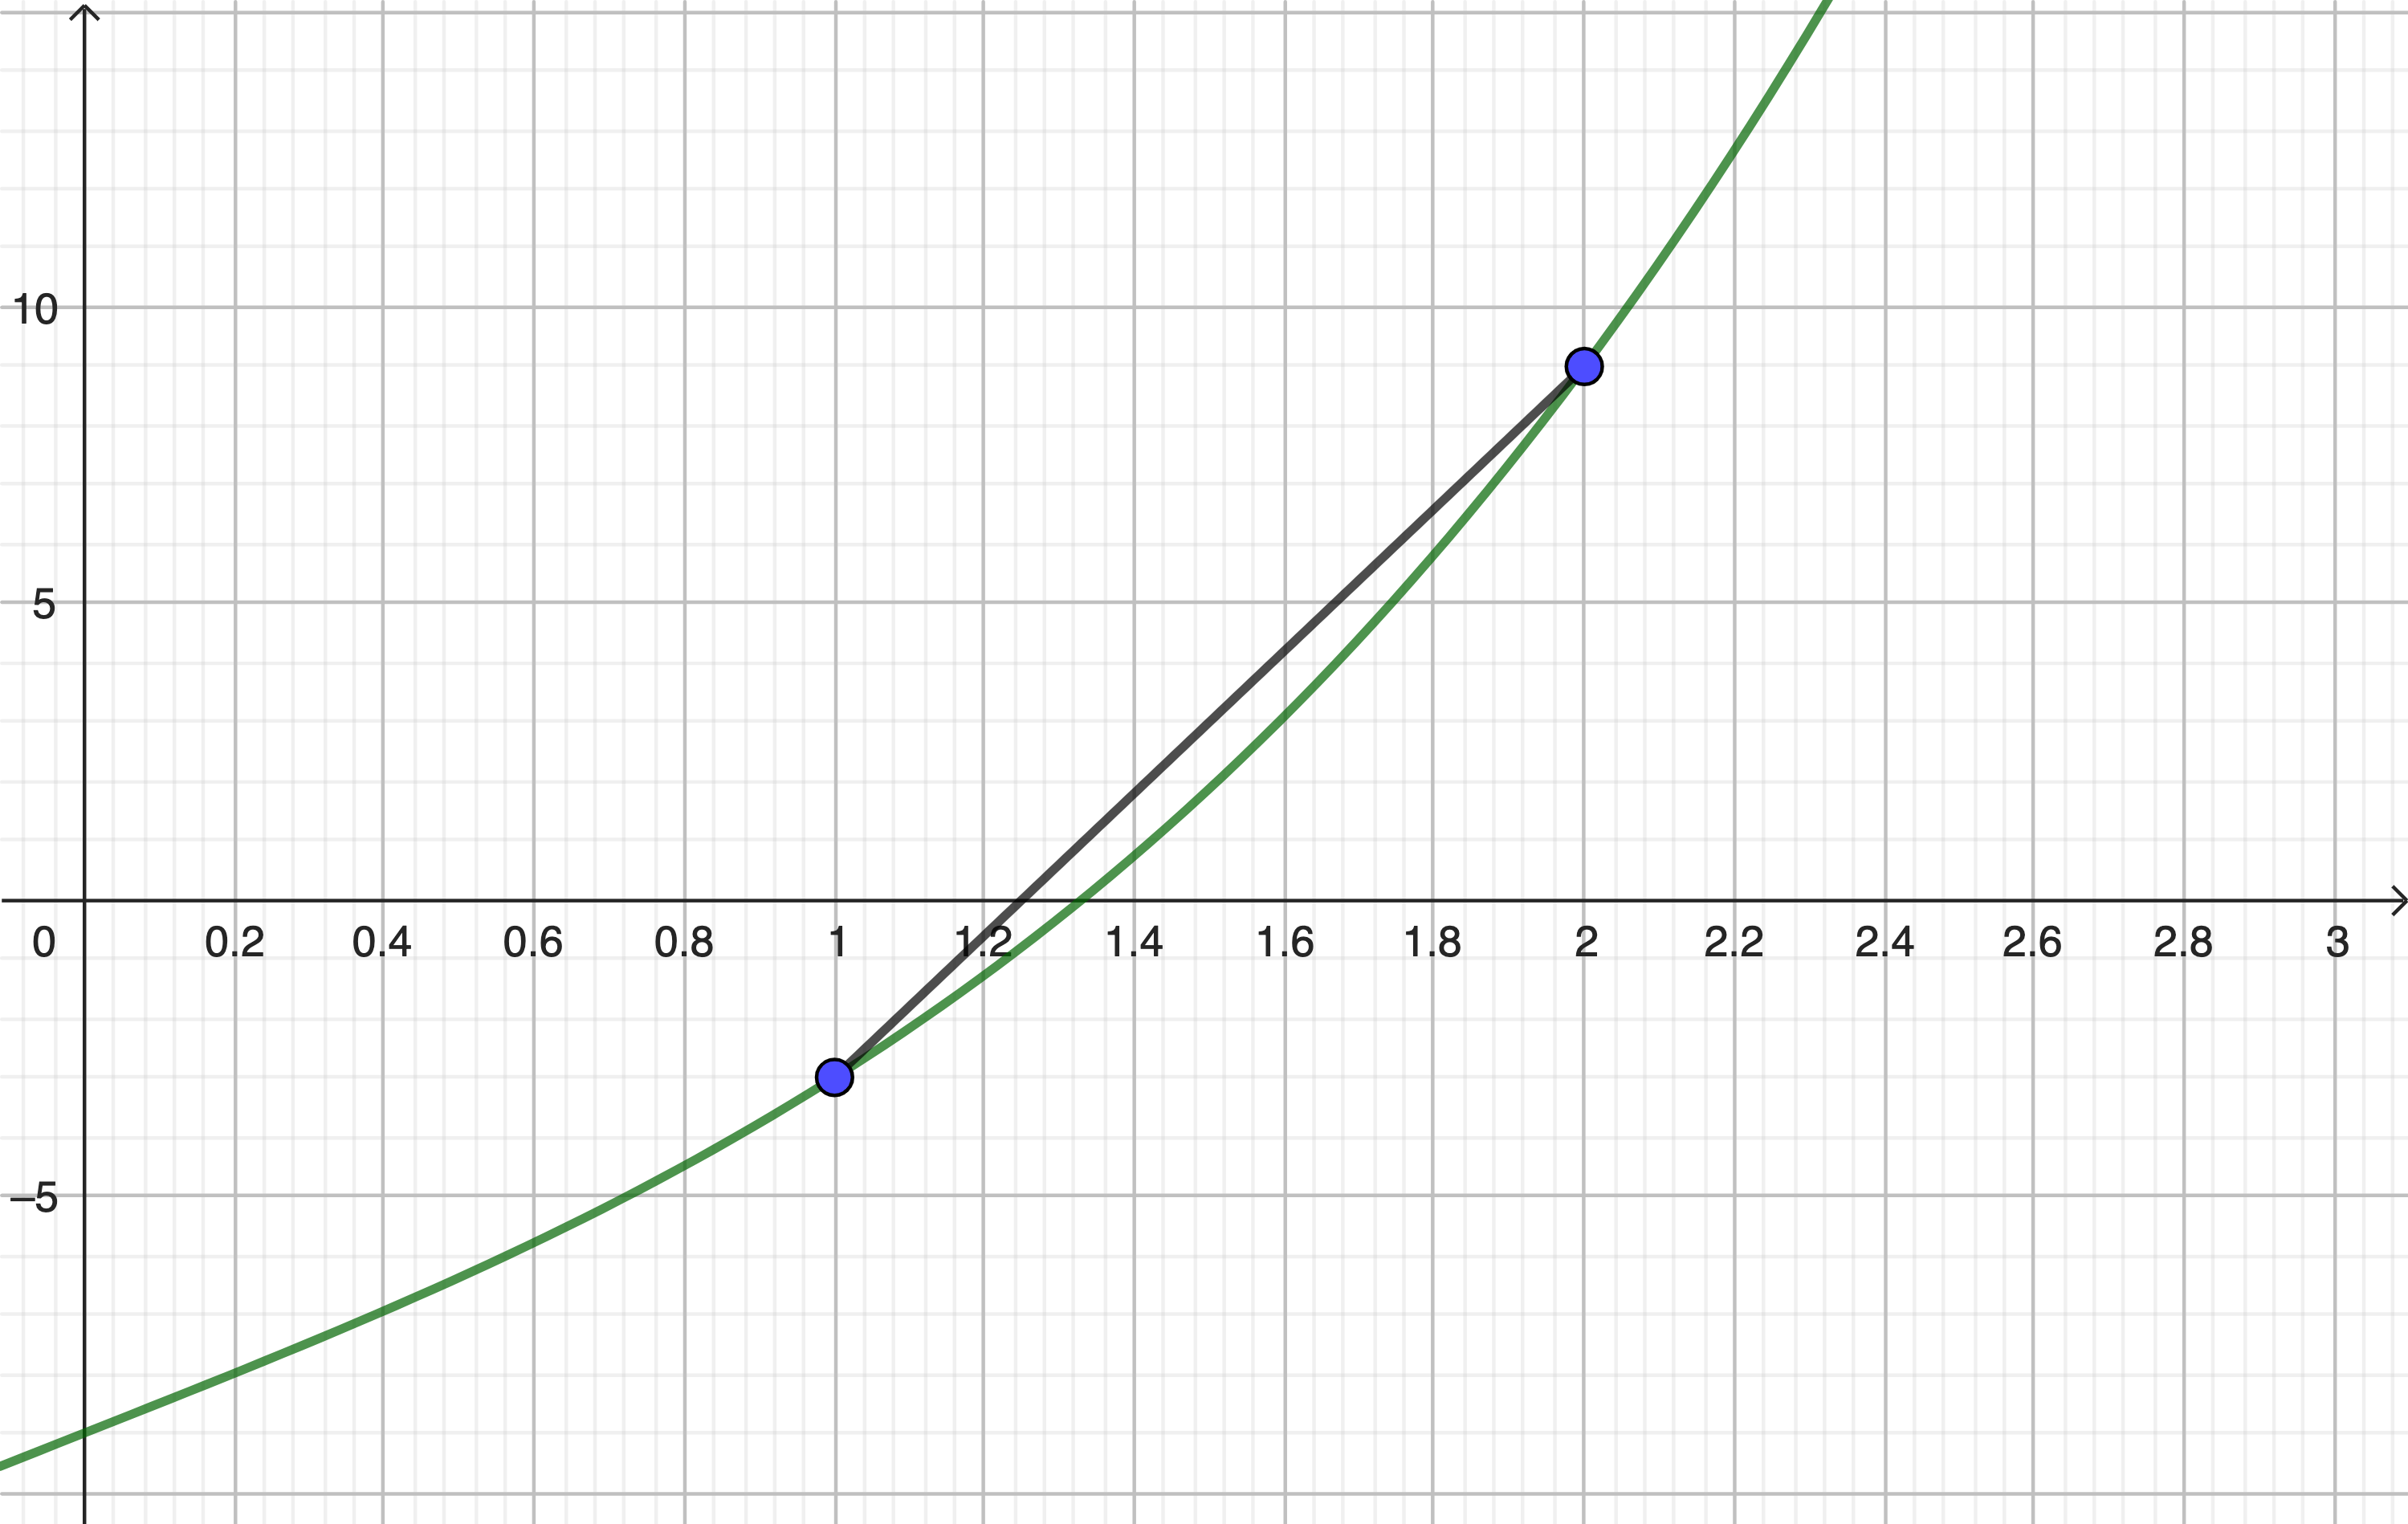
\includegraphics[width = 0.5 \textwidth]{media/bsp_Lineare_Interpolation.png}
	\end{center}
	Mit der Steigung können wir die Nullstelle der Verbindungsgerade einfach berechnen.
	\begin{center}
		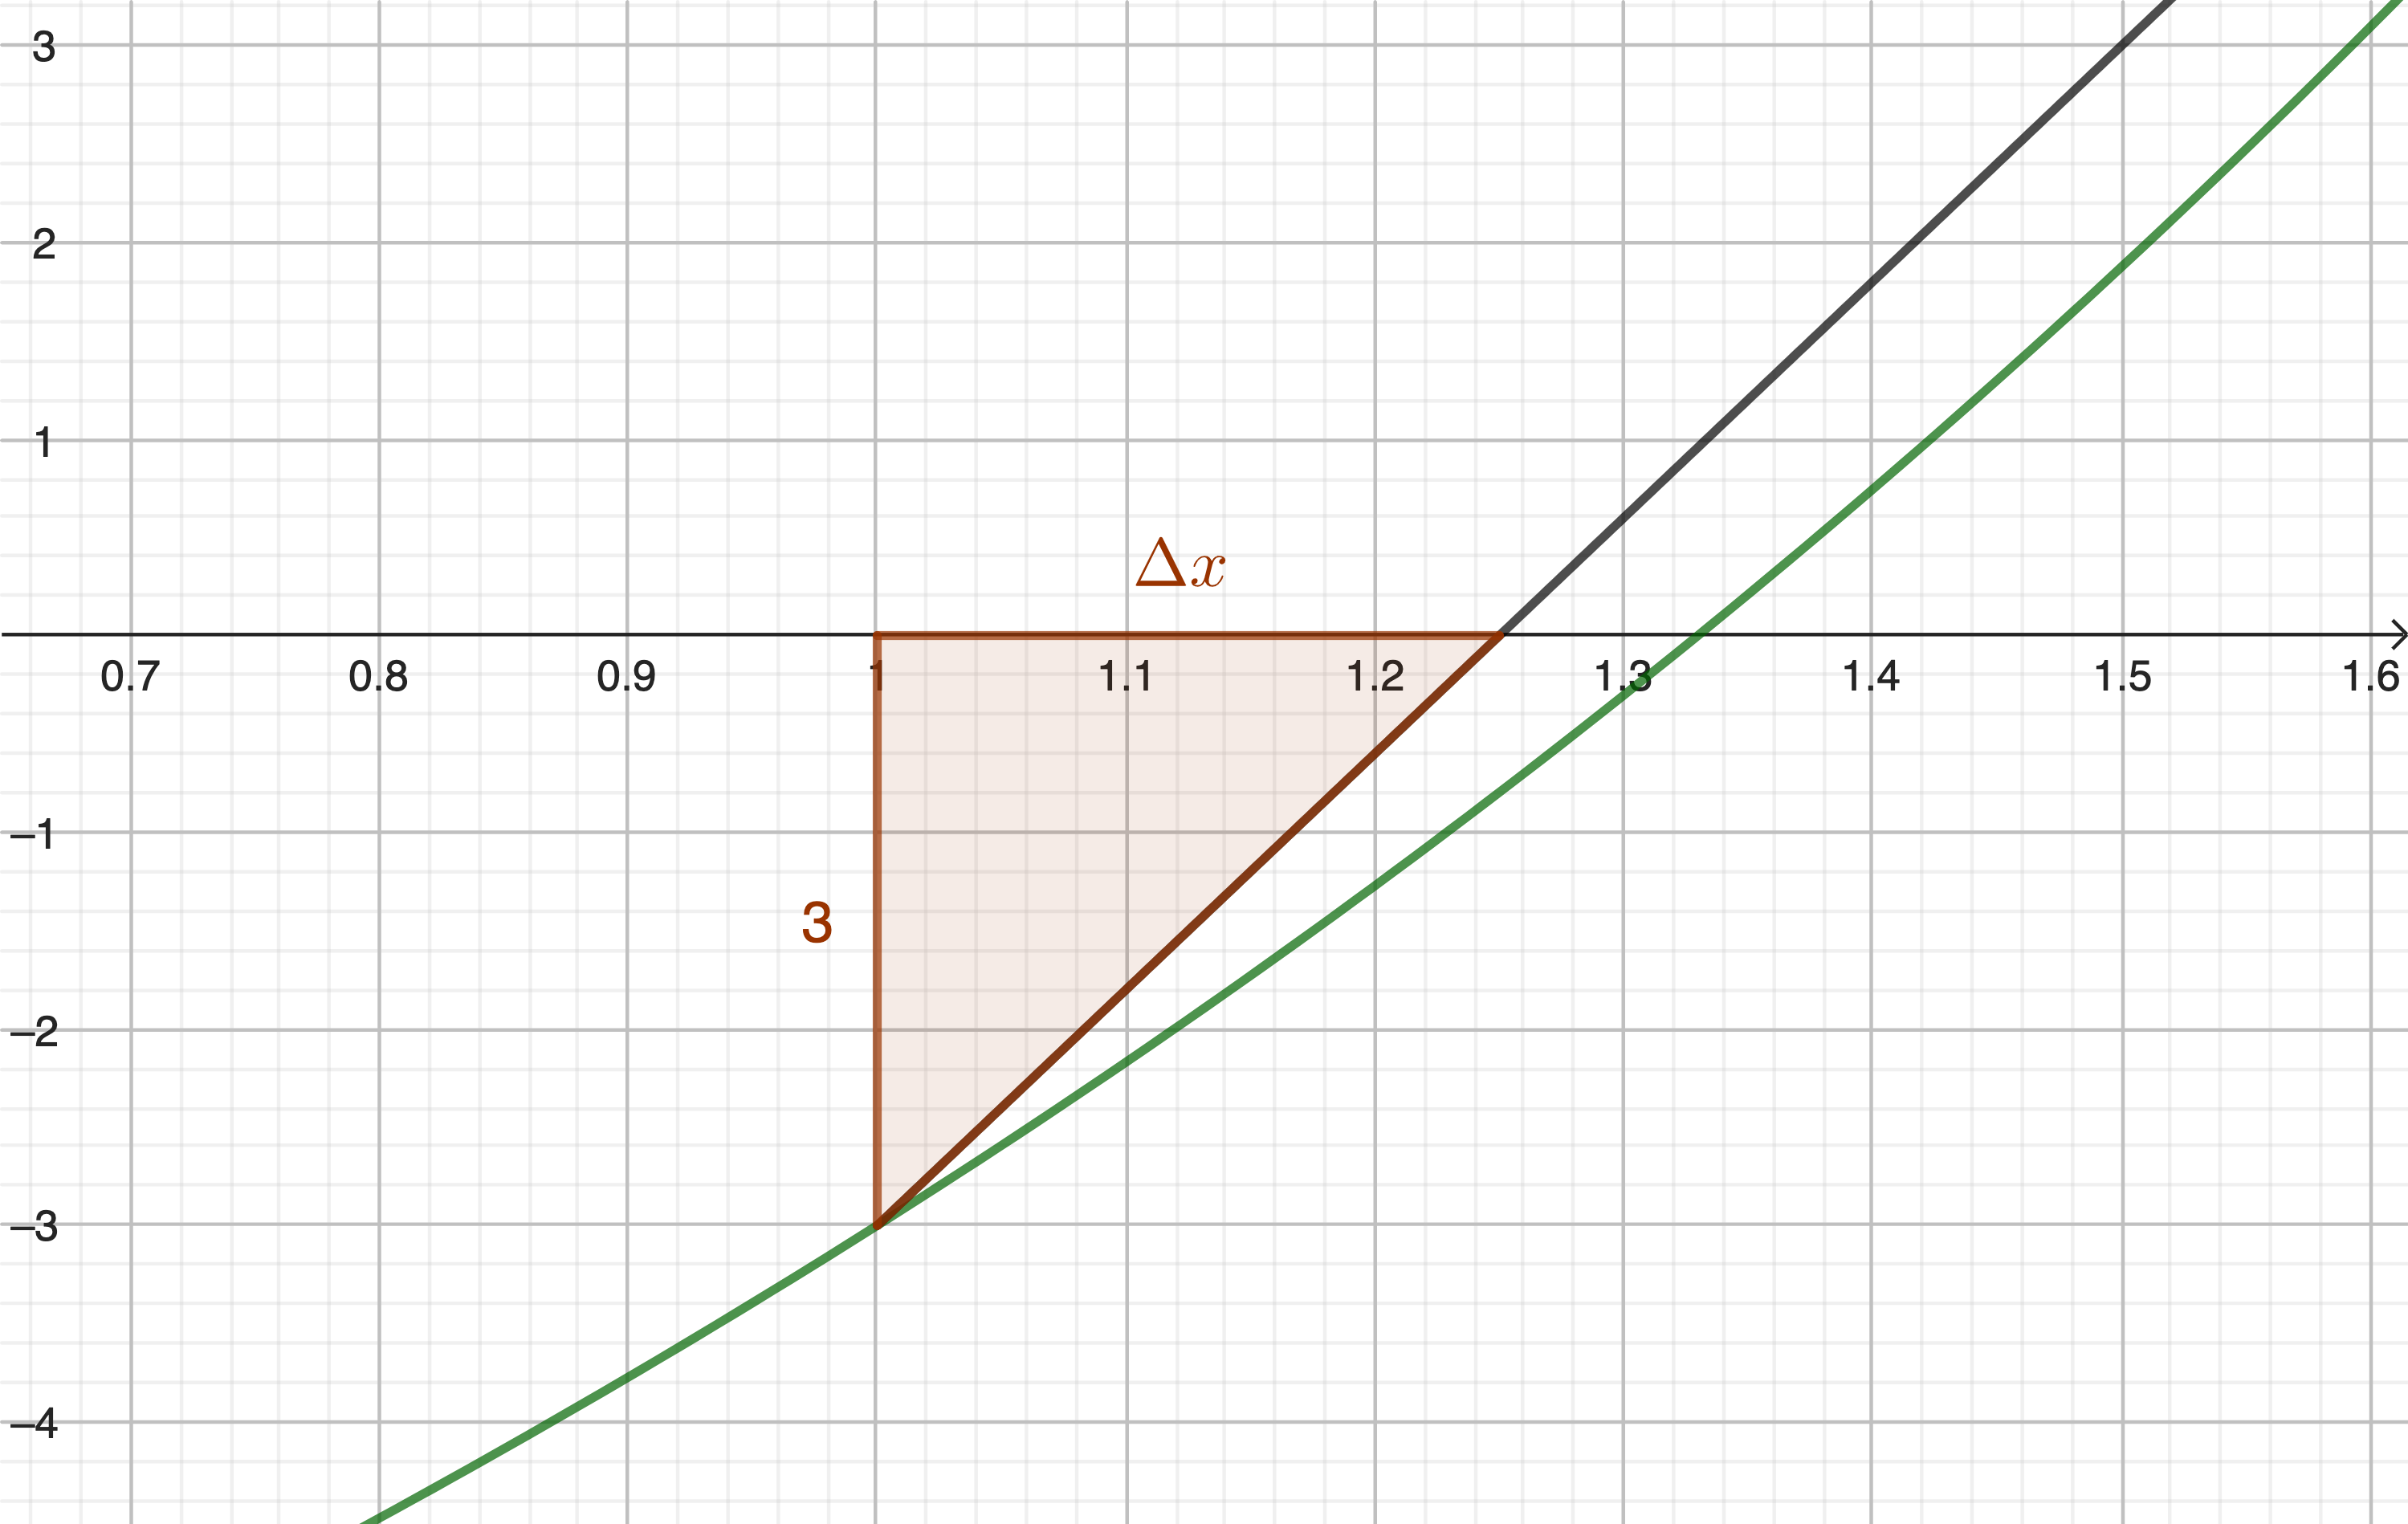
\includegraphics[width = 0.5 \textwidth]{media/bsp_Lineare_Interpolation-Dreieck.png}
	\end{center}
	Es gilt:
	\[ \frac{0-(-3)}{\Delta x} = 12 \iff \Delta x = \frac{3}{12} \Longrightarrow x_0 \approx 1+\Delta x = 1.25\]
	An der Stelle $x=1.25$ gilt $f(1.25) = -0.796875 < 0$. Demnach ist die Nullstelle im Bereich $1.25 < x_0 < 2$.

	Wieder wird dieses Verfahren mehrfach wiederholt:

	\begin{itemize}
		\item Die Gerade zwischen den Punkten $(1.25, -0.796875)$ und $(2,9)$ hat die Steigung
		      \[m = \frac{9-(-0.796875)}{2-1.25} = 13.0625\]
		      Die Verbindungsgerade schneidet die $x$-Achse an der Stelle
		      \[1.25 - \frac{-0.796875}{m} = 1.311004785\]
		      Weil $f(1.311004785)\approx -0.2 <0$ ist, liegt die Nullstelle im Intervall $[1.311004785, 2]$.
		\item Die Gerade zwischen den Punkten $(1.311004785, -0.19170818)$ und $(2,9)$ hat die Steigung
		      \[m = \frac{9-(-0.19170818)}{2-1.311004785} = 13.34074311\]
		      Die Verbindungsgerade schneidet die $x$-Achse an der Stelle
		      \[1.311004785 - \frac{-0.191708172}{m} = 1.325374912\]
		      Weil $f(1.325374912)\approx -0.04 <0$ ist, liegt die Nullstelle im Intervall $[1.325374912, 2]$.
	\end{itemize}
	Nach diesen drei Schritten erhält man mit $x\approx 1.325374912$ eine Approximation, die bereits sehr nahe an der Nullstelle liegt.

\end{bsp}

Im Vergleich zum Bisektionsverfahren liefert die Regula Falsi häufig deutlich bessere Näherungen. Allerdings ist die Verbesserung nicht garantiert und hängt vom Verlauf der Funktion ab. Ausserdem kann man im Unterschied zum Bisektionsverfahren, die Genauigkeit nicht mehr gut Abschätzen.

Allgemein formuliert lässt sich die jeweils nächste Näherung mit folgenden Schritten berechnen: Seien $(a,f(a))$ und $(b, f(b))$ die aktuellen Punkte auf der Kurve, zwischen denen sich die Nullstelle befindet.
\begin{enumerate}
	\item Die Steigung $m$ zwischen den beiden Punkten ist
	      \[m = \frac{f(b)-f(a)}{b-a}\]
	\item Die nächste Approximation für die Nullstelle ist
	      \[x = a - \frac{f(a)}{m}\] %= a - f(a)\frac{b-a}{f(b)-f(a)}
\end{enumerate}

\begin{ueb}
	{}{}
	\begin{enumerate}
		\item Führen Sie drei Schritte der Regula Falsi durch, um die Lösung der Gleichung
		      \[x^3 = 7-5x\]
		      im Intervall $1<x<2$ zu finden.
		\item Die Funktion \texttt{num-solv} des Taschenrechners funktioniert vermutlich nach einem ähnlichen Verfahren, wobei Texas Instruments den genauen Algorithmus nicht preisgibt. Testen Sie die Taschenrechner-Funktion
		      \begin{enumerate}
			      \item Mit der Gleichung  \(x^3 = 7-5x\) von oben. Verwenden Sie $x=1$ als Startwert.
			      \item Mit der Gleichung \(x^2 = 0\). Verwenden Sie wieder $x=1$ als Startwert. Geben Sie eine Vermutung, wieso die Taschenrechner-Funktion versagt.
		      \end{enumerate}
		\item Schreiben Sie ein Programm, das die Regula Falsi implementiert. Halten Sie sich an die Vorlage in \Cref{uebng:bisektion}. Testen Sie Ihr Programm anschliessend mit den Zahlen aus dem \Cref{bsp:intro-lineareInterpolation}.
	\end{enumerate}
\end{ueb}

\clearpage
\emph{Lösungen}
\begin{enumerate}
	\item 1.1161986788354266
	\item  \begin{enumerate}
		      \item Der Taschenrechner liefert $x=1.119437527$.
		      \item \dots %Der Taschenrechner meldet einen Fehler. Vermutlich werden verschiedene Stellen getestet. Weil aber jeder Output positiv ist (mit Ausnahme von $x=0$), werden keine zwei Stellen gefunden, deren Output unterschiedliche Vorzeichen haben.
	      \end{enumerate}
	\item Mögliche Lösung:
	      \lstinputlisting[language=Python]{Programme/regula-falsi.py}
\end{enumerate}

















\clearpage
\subsection{Newton-Verfahren}
Obwohl die Regula Falsi bereits viel schneller als die Bisektion zu guten Näherungen führt, beachtet sie noch nicht die Form des Graphen von $f(x)$.

tbc